\documentclass{article}
\usepackage{amsmath, amsthm, amssymb, amsfonts, bm}
\usepackage{graphicx}
\usepackage[T1]{fontenc}
\usepackage[utf8]{inputenc}
\usepackage[a4paper]{geometry}
\usepackage{fancyhdr}
\usepackage[algo2e]{algorithm2e}
\fontfamily{cmr}

\title{DD2424 - Assignment 1 (Bonus)}
\author{Oskar Stigland \\ stigland@kth.se}

\pagestyle{fancy}
\fancyhf{}
\rhead{stigland@kth.se}
\lhead{DD2424 - Deep Learning in Data Science}
\rfoot{Page \thepage}

\begin{document}
%\maketitle

	\begin{titlepage}
		\begin{center} 
			
			\rule{\linewidth}{0.5mm}\\[0.5 cm]
			{ \huge \bfseries DD2424 - Assignment 1 (Bonus)}\\[0.3 cm] % Title of your document
			\rule{\linewidth}{0.5mm}\\[1 cm]
					
			\small\vfill
			\begin{center}
			\centering
			{\large \bfseries \textsc{Summary}}\\
			\vspace{1cm}
			\begin{minipage}{8cm}
				
				I have completed both parts of the bonus assignment exercises. For the first part, I have used the entirety of the training data, implemented training data augmentation, and used a decaying learning rate. I also experimented with a numer of different values for the regularization parameter. For the second part, I have derived the gradients for the multiple binary cross-entropy loss and compared the results of using the sigmoid activation with the corresponding results for the softmax.
			\end{minipage}
			\end{center}
			\large\vfill
						

		\end{center}	
		
		\begin{minipage}{0.4\textwidth}
			\begin{flushleft} \large
				%\emph{Student:}\\
				Oskar \textsc{Stigland}\\
				DD2424\\
				Spring 2023
			\end{flushleft}
		\end{minipage}	

	\end{titlepage}

\newpage
\section*{Part I - Improving Performance of the Network}
	For this part, I have experimented with different parameter setting while adding the improvements. I recorded the best results and the (seemingly) most stable training procedure with the following parameter settings:
	\begin{itemize}
		\item \texttt{batchN} = 50
		\item \texttt{epochsN} = 50
		\item $\lambda = 0.1$
		\item $\eta = 0.01$
		\item $\eta_n = 10$
		\item $p_{\text{flip}} = 0.2$
	\end{itemize}
	where the $\eta_n$ corresponds to the number of epochs per decay of the learning rate. Per the assignment suggestion, I initially used a horizontal flip probability of $p = 0.5$ for the training data, performing a shuffle and flip for every epoch. However, it seems a lower flip probability works equally well and I thus settled for $p = 0.2$. As mentioned, I have also utilized all of the tranining data, reducing the validation data to a smaller subset of the training data with $N_{\text{val}} = 1000$. I also experimented with a number of different settings for the regularization parameter. It wuold seem $\lambda = 0.1$ is a fairly optimal value for training. For the above parameters, the model reaches an accuracy of $40.76$\%.

	\begin{figure}[h!]
		\centering
		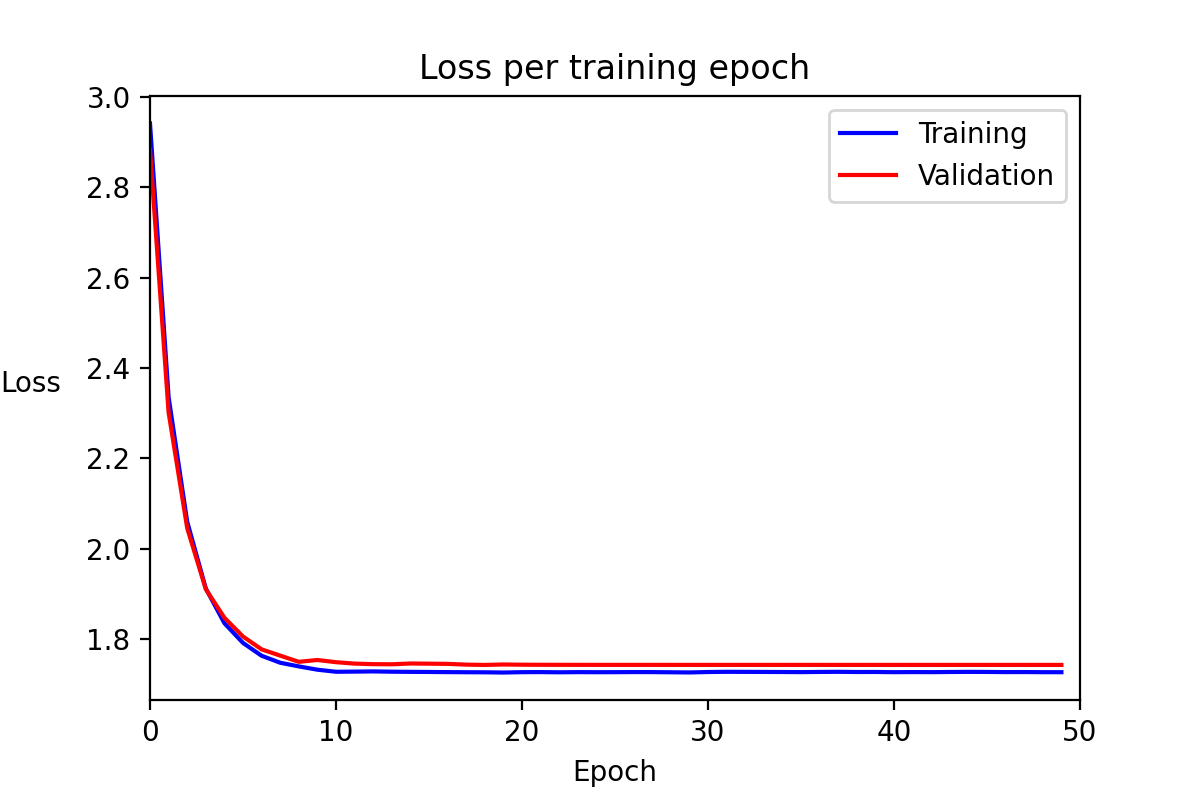
\includegraphics[width=7cm]{../plots/loss_v5.png}
		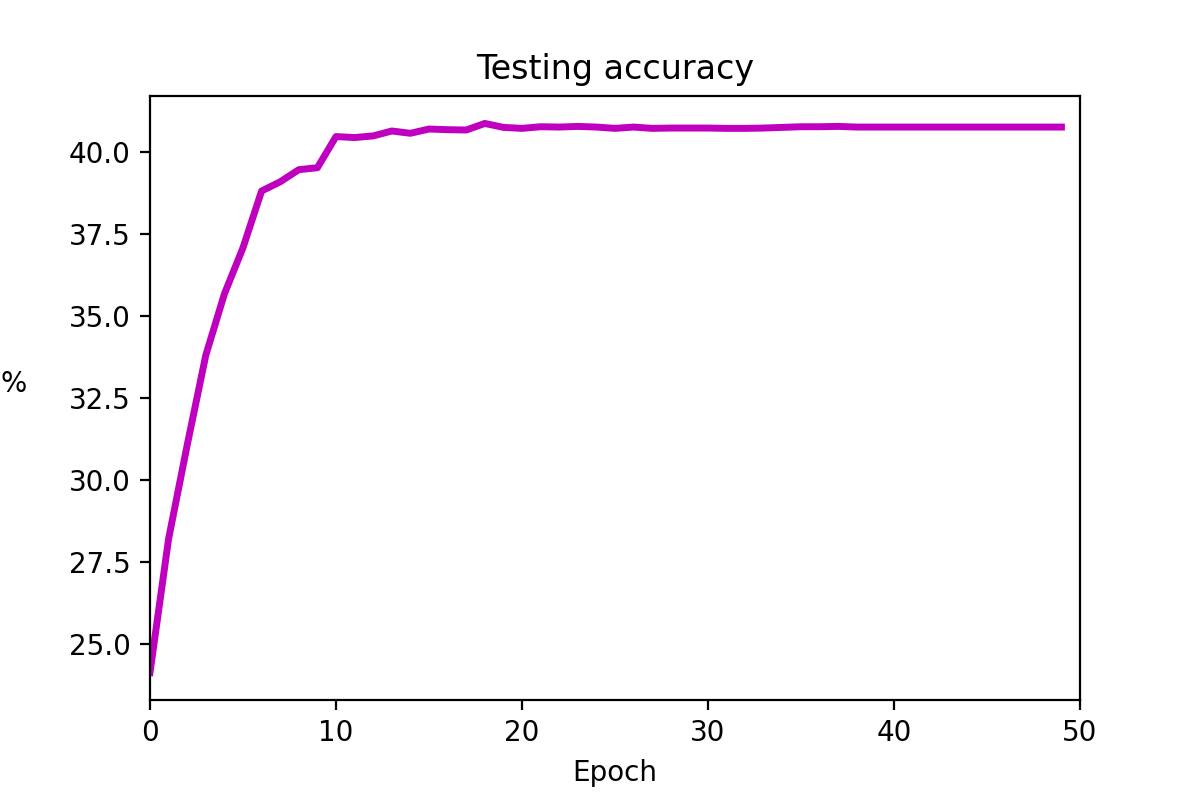
\includegraphics[width=7cm]{../plots/acc_v5.png}
		\caption{Loss and accuracy for optimal set of parameters}
		\vspace{0.2cm}
		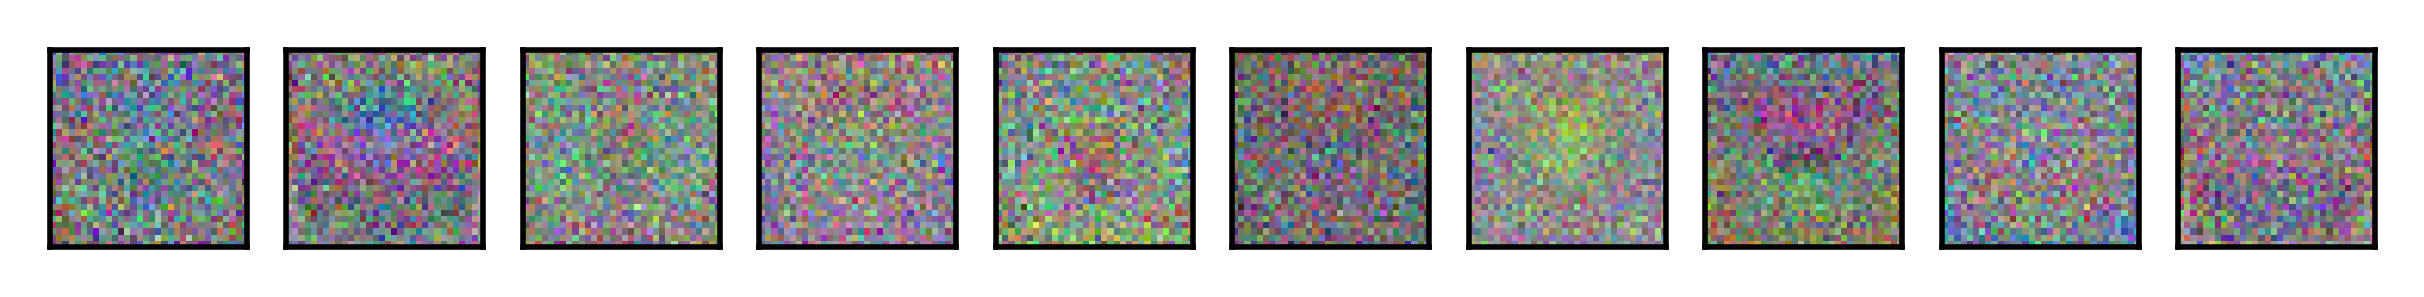
\includegraphics[width=12cm]{../plots/weights_v5.png}
		\caption{Class-specific weights for optimal set of parameters}
		%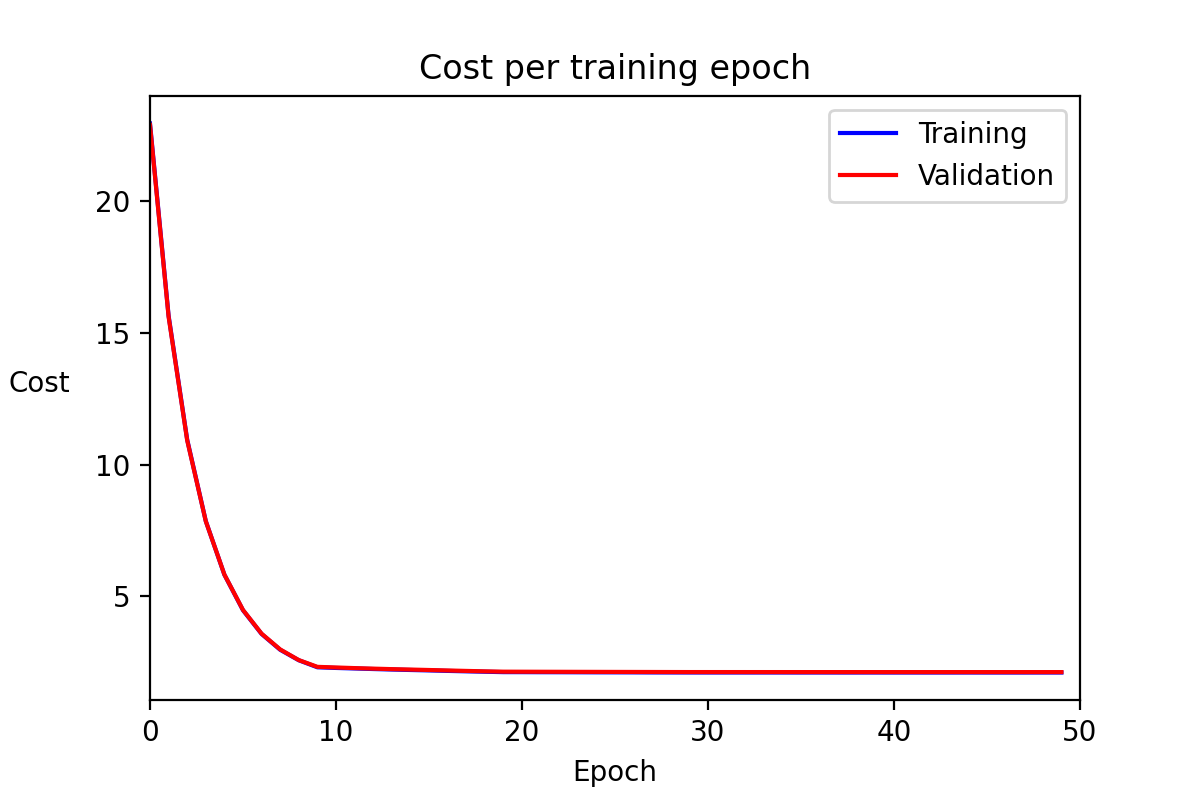
\includegraphics[width=7cm]{../plots/cost_v2.png}	
	\end{figure}


\newpage
\section*{Part II - Multiple Binary Cross-Entropy Losses}
\vspace{0.5cm}
\subsection*{Obtaining the gradient}
	In order to obtain the expression for $\partial\ell/\partial\bm{s}$, we consider the chain rule, where
	$$\dfrac{\partial\ell}{\partial\bm{s}} = \dfrac{\partial\ell}{\partial\bm{p}}\dfrac{\partial\bm{p}}{\partial\bm{s}}$$
	First, we considering differentiating the class-specific loss w.r.t. the correspoding probability, s.t. $\ell = -1/K \sum_{k=1}^K \ell_k$:
		$$\dfrac{\partial\ell_k}{\partial p_k} = \frac{\partial}{\partial p_k} \left[ (1 - y_k)\log(1 - p_k) + y_k \log(p_k)\right] = \frac{y_k - 1}{1 - p_k} + \frac{y_k}{p_k} $$
	Second, we recognize that $p_k = \sigma(s_k)$, wherer $\sigma: \mathbb{R} \rightarrow [0, 1]$ is the logistic sigmoid function, for which we also have that
	$$\sigma(s) = \frac{1}{1 + e^{-s}} = \frac{e^{s}}{e^{s} + 1}$$
	as well as $1 - \sigma(s) = \sigma(-s)$ and $\sigma'(s) = \sigma(s)(1 - \sigma(s))$. Hence, we get that
	\begin{align*}
		\dfrac{\partial \ell_k}{\partial s_k} &=  \frac{\partial}{\partial s_k} \left[ (1 - y_k)\log(1 - \sigma(s_k)) + y_k \log(\sigma(s_k))\right] \\
		&=\frac{y_k - 1}{1 - \sigma(s_k)}\sigma(s_k)(1 - \sigma(s_k)) + \frac{y_k}{\sigma(s_k)}\sigma(s_k)(1 - \sigma(s_k)) \\
		&=  (y_k - 1)\sigma(s_k) + y_k(1 - \sigma(s_k) \\
		&=  y_k - \sigma(s_k)  
	\end{align*}
	Hence, the Jacobians we're looking for are given by
	\begin{align*}
		\dfrac{\partial\ell}{\partial \bm{p}} &= -\frac{1}{K}\left[\bm{y}^T\text{diag}(\bm{p})^{-1} - (\bm{1} - \bm{y})^T \text{diag}(\bm{1} - \bm{p})^{-1}\right]\\
		\dfrac{\partial\bm{p}}{\partial \bm{s}} &= \text{diag}(\bm{p})\,\text{diag}(\bm{1} - \bm{p})
	\end{align*}
	such that
	\begin{align*}
		\dfrac{\partial\ell}{\partial \bm{s}} &= -\frac{1}{K}\left[\bm{y}^T\underbrace{\text{diag}(\bm{p})^{-1}\text{diag}(\bm{p})\,\text{diag}(\bm{1} - \bm{p})}_{=\text{diag}(\bm{1} - \bm{p})} -  (\bm{1} - \bm{y})^T \underbrace{\text{diag}(\bm{1} - \bm{p})^{-1}\text{diag}(\bm{p})\,\text{diag}(\bm{1} - \bm{p})}_{=\text{diag}(\bm{p})}  \right]\\
		&= -\frac{1}{K}\left[ \bm{y}^T\text{diag}(\bm{1} - \bm{p}) - (\bm{1} - \bm{y})^T\text{diag}(\bm{p})\right] \\
		&= -\frac{1}{K}\left[\bm{y} - \bm{y}^T\text{diag}(\bm{p}) - \bm{p} + \bm{y}^T\text{diag}(\bm{p}) \right] \\
		&= -\frac{1}{K}(\bm{y} - \bm{p})
	\end{align*}
	Hence, using the result from the previous loss, we should have that
	$$\dfrac{\partial\ell}{\partial \bm{W}} = -\frac{1}{K}(\bm{y} - \bm{p})\,\bm{x}^T, \quad \dfrac{\partial\ell}{\partial \bm{b}} = -\frac{1}{K}(\bm{y} - \bm{p})$$

\newpage
\subsection*{Results}

%\section*{Theory}
%\subsection*{Task 1}
%	We want to prove that the expectation maximization algorithm decreases the energy,
%	$$E(\bm{\mu}, \bm{r}) = \sum_{n=1}^{N}\sum_{k=1}^K \vert\vert\bm{x}_n - \bm{\mu}_k\vert\vert^2 r_{k, n},$$
%	at every step. In the first step we choose the means for every cluster such that
%	$$\bm{\mu}_k = \frac{\sum_n r_{k, n}\bm{x}_n}{\sum_{n}r_{k, n}}$$
%	and in the second step we assign the points $\bm{x}_1, \bm{x}_2, \dots, \bm{x}_N$ to clusters by minimizing the euclidean distance between a point and it's cluster mean:
%	$$r_{k, n} = \begin{cases}
%		1 \quad\text{if}\quad k = \arg\min_j \vert\vert \bm{x}_n - \bm{\mu}_j\vert\vert^2 \\
%		0 \quad\text{otherwise}
%	\end{cases}$$
%	\begin{itemize}
%		\item[(i)] We assume that the points are already assigned to different clusters. Hence, for every cluster $\mathcal{C}_k$ we want to choose $\bm{\mu}_k$ such that we minimize
%		$$E_k(\bm{\mu}_k) = \sum_{\bm{x}_n\in \mathcal{C}_k} \vert\vert \bm{x}_n - \bm{\mu}_k\vert\vert^2$$
%		It suffices to note that this is achieved by picking $\tilde{\bm{\mu}}$ such that
%		$$\nabla_{\mu}E_k(\tilde{\bm{\mu}}) = \bm{0} \implies \tilde{\bm{\mu}} = \frac{\sum_nr_{k, n}\bm{x}_n}{\sum_n r_{k,n}}$$
%		We also know that $E_k(\bm{\mu})$ defines a \textbf{convex} optimization problem since $f(x) = x^2$ is a convex function, i.e. $f''(x) > 0$, $\forall\,x\in\mathcal{D}_f$, and we have that 
%		$$E_k(\bm{\mu}_k) = \sum_{\bm{x}_n\in \mathcal{C}_k}f(\vert\vert\bm{x}_n - \bm{\mu}_k\vert\vert)$$
%		meaning that $E_k$ is also a convex function since $\mathcal{D}_f = \mathbb{R}$ and $\vert\vert\bm{x}_n - \bm{\mu}_k\vert\vert \in\mathbb{R}$, $\forall\,\bm{x}_n, \bm{\mu}_k$. Thus, we must have that
%		$$E_k(\bm{\mu}) \leq E_k(\tilde{\bm{\mu}})$$
%		for every update $\tilde{\bm{\mu}}$. Hence, if the algorithm hasn't already converged, this step will minimize the total energy.
%		\item[(ii)] The argument for this step is trivial. By the definition of $r_{k, n}$ above this step must mean that the energy for the updated cluster assignments is less than or equal to the previous energy. 
%	\end{itemize}
%
%\subsection*{Task 2}
%	For the first step we find the position of $k$ centroids. For every centroid, we are multiplying $n$ elements and then summing $n$ elements. Then we are summing $n$ more elements and finally dividing the two sums. Hence, we have
%	$$\mathcal{O}(k(n + 2(n-1) + 1)) = \mathcal{O}(k(3n + 1))$$
%	operations. For the second step, we are evaluating $n$ points and their cluster assignments. For each point, we need to compute $k$ distances, which amounts to taking $d$ (i.e. the number of dimensions) differences, $d$ squares, $d - 1$ sums and then squaring. Hence, we would need 
%	$$\mathcal{O}(nk(3d - 1))$$
%	computations. Technically, we would also need to make some number of comparisons at every step to find the proper cluster assignment, but this would depend on the algorithm used for comparing and sorting the differences. 
%	
%	
%\subsection*{Task 3}
%	We want to prove that the function
%	$$J(\bm{\mu}) = \sum_{n=1}^N \min_{1\leq j\leq k} \vert\vert\bm{x}_n - \bm{\mu}_j\vert\vert^2$$
%	is \textbf{not convex}. We say that a function $f$ is convex if and only if 
%	$$\alpha f(x_1) + (1 - \alpha)f(x_2) \geq f(\alpha x_1 + (1 - \alpha)x_2), \quad \forall\,x_1,x_2\in\mathcal{D}_f \quad\aand\quad \forall\,\alpha\in[0, 1]$$
%	Hence, we want to find a counterexample. We look at $\alpha = \frac{1}{2}$ and want to show that
%	$$\frac{1}{2}\left(J(\bm{\mu}^{(1)}) + J(\bm{\mu}^{(2)})\right) \leq J\left(\frac{1}{2}(\bm{\mu}^{(1)} + \bm{\mu}^{(2)})\right)$$
%	for some $\bm{\mu}^{(1)}$, $\bm{\mu}^{(2)}$. Hence, we want to show that
%	$$\frac{1}{2}\left(\sum_{n=1}^N \min_{1\leq j\leq k}\vert\vert\bm{x}_n - \bm{\mu}^{(1)}_j\vert\vert^2 + \sum_{n=1}^N\min_{1\leq j\leq k}\vert\vert\bm{x}_n - \bm{\mu}^{(2)}_j\vert\vert^2\right) \leq \sum_{n=1}^N \min_{1\leq j\leq k}\bigg\vert\bigg\vert \bm{x}_n - \frac{1}{2}\left(\bm{\mu}^{(1)}_j + \bm{\mu}^{(2)}_j\right)\bigg\vert\bigg\vert^2$$
%	We have a finite set of points
%	$$D = \{\bm{x}_1, \bm{x}_2, \dots, \bm{x}_N\} \subset\mathbb{R}^d$$
%	and two \textbf{matrices} of centroids $\bm{\mu}^{(1)}$, $\bm{\mu}^{(2)}$. We set 
%	$$\bm{\mu}_1^{(1)} = \bm{x}_1 \quad\aand\quad \bm{\mu}_j^{(1)} \neq \bm{x}_1 \quad j = 2, 3, \dots, k$$
%	and
%	$$\bm{\mu}_2^{(2)} = \tilde{\bm{x}} \quad\text{s.t.}\quad \bigg\vert\bigg\vert\tilde{\bm{x}} - \frac{1}{N}\sum_{n=1}^{N}\bm{x}_n\bigg\vert\bigg\vert^2 \geq \alpha\cdot\left(\arg\max_{\bm{x}\in D}\bigg\vert\bigg\vert \bm{x} -  \frac{1}{N}\sum_{n=1}^N\bm{x}_n\bigg\vert\bigg\vert^2\right)$$
%	for some sufficiently large constant $\alpha > 0$. That is, such that $\tilde{\bm{x}}$ is so far away that we would never choose to pair any observation with it. We also set $\bm{\mu}_j^{(2)} = \bm{\mu}_j^{(1)}$ for $j = 2, 3, \dots, k$. Since for all $\bm{x}\in D$ we have that
%	$$\vert\vert \bm{x} - \bm{\mu}_1^{(2)}\vert\vert^2 > \min_{1\leq j\leq k}\vert\vert \bm{x} - \bm{\mu}_j^{(2)}\vert\vert \quad\aand\quad \vert\vert \bm{x} - \frac{1}{2}\left(\bm{\mu}_1^{(1)} +  \bm{\mu}_1^{(2)}\right)\vert\vert^2 > \min_{1\leq j\leq k}\vert\vert \bm{x} - \bm{\mu}_j^{(2)}\vert\vert$$
%	from which it follows that
%	$$J(\bm{\mu}^{(2)}) = J\left(\frac{1}{2}\bm{\mu}^{(1)} + \frac{1}{2}\bm{\mu}^{(2)}\right)$$
%	since the with exception of the first centroid the two centroid matrices $\bm{\mu}^{(1)}$ and $\bm{\mu}^{(2)}$ are equal, while $\bm{\mu}_1^{(2)}$ is so far away from the observations that we will still pick some other centroid than the average of the two first centroids in $\bm{\mu}^{(1)}$ and $\bm{\mu}^{(2)}$. Now, we realize that we must have that
%	$$J(\bm{\mu}^{(1)}) \leq J(\bm{\mu}^{(2)})$$
%	since for $\bm{x}_1$ we'll have that
%	$$\min_{1\leq j\leq k}\vert\vert\bm{x}_1 - \bm{\mu}_j^{(1)}\vert\vert^2 = 0 \quad\aand\quad \min_{1\leq j\leq k}\vert\vert \bm{x}_1 - \bm{\bm{\mu}}_1^{(2)}\vert\vert^2 \geq \min_{2\leq j\leq k}\vert\vert\bm{x}_1 - \bm{\mu}_j^{(2)}\vert\vert^2 \geq 0$$
%	while for all the other points $\bm{x}\in D\setminus\bm{x}_1$ the euclidean distances will be identical (or we will have points such that we choose $\bm{\mu}_1^{(1)}$, meaning that the distance will be strictly smaller), meaning that
%	$$J(\bm{\mu}^{(2)}) = \frac{1}{2}J(\bm{\mu}^{(2)}) + \frac{1}{2}J(\bm{\mu}^{(2)}) \geq \frac{1}{2}J(\bm{\mu}^{(1)}) + \frac{1}{2}J(\bm{\mu}^{(2)})$$
%	$$\iff  J\left(\frac{1}{2}\bm{\mu}^{(1)} + \frac{1}{2}\bm{\mu}^{(2)}\right) \geq \frac{1}{2}J(\bm{\mu}^{(1)}) + \frac{1}{2}J(\bm{\mu}^{(2)})$$
%	Hence, the function is \textbf{not convex}. '
%	
%\newpage
%\section*{Experiments}
%
%\subsection*{Task 4}
%	The code is presented on the last pages.
%	
%\subsection*{Task 5}
%	Using the Forgy method for $100$ iterations I got an \textbf{average} purity of $0.89$, while for the random partition method I got an \textbf{average} purity of $0.78$. Hence, the Forgy method actually performs significantly better on average. 
%	
%\subsection*{Task 6}
%	Projecting the dataset onto its first two principal components I get the following plot:
%	\begin{figure}[h]
%		\centering
%		\includegraphics[width=10cm]{irisprojection.png}
%	\end{figure}\\
%	From this plot, we can clearly see that the first class of Iris flowers form a distinct cluster when projected onto the first two principal components. We can also see that the second and third classes overlap a bit, which should explain why when using the Forgy method we get an average purity of something like $0.9$. That is, for the first class we should have more or less perfect clustering, while we have a small overlap for the second and third. For some iterations the Forgy method actually achieved a purity of $0.98$. 
%
%
%
%
%\newpage
%
%	\begin{figure}[h]
%		\centering
%		\includegraphics[width=18cm]{kmeanscode1.pdf}
%	\end{figure}
%	\begin{figure}[h]
%		\centering
%		\includegraphics[width=18cm]{kmeanscode2.pdf}
%	\end{figure}


\end{document}